\documentclass[11pt]{article}
%Gummi|063|=)
\title{\textbf{Concept and Methodology}}
\author{Deebul Nair}
\date{\today}
\usepackage{graphicx}
\usepackage{amsfonts}
\usepackage{amsmath}

\begin{document}
\maketitle
\section{Introduction}

\begin{figure}[htp]
\centering
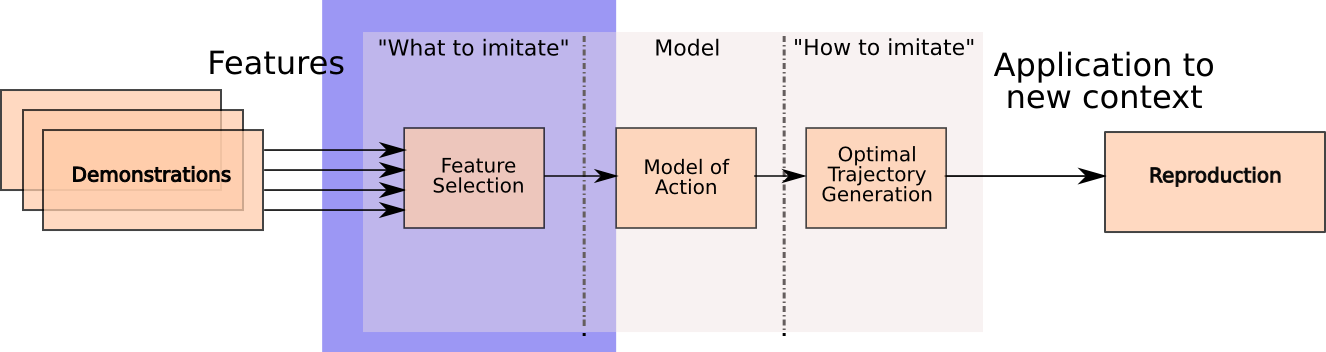
\includegraphics[scale=0.4]{/data/dataDeebul/rnd/RecommenderSystemInRobotics/art/myRnD.png}
\caption{Learning by Demonstration}
\label{Figure }
\end{figure}

Information Theory can be used as the basis for some of the learning models. In this the rnd we would use the concepts rooted in Information theory to model the action for learning actions from demonstrations. 
This section introduces the some of the basic concepts of Information theory.

The following concepts related to Information theory are discussed :
\begin{itemize}
	\item Entropy
	\item Differential Entropy
	\item Maximum-Entropy principle
	\item Mutual information between a pair of random variables
	\item Kullback-Leibler divergence
	\item Copulas
\end{itemize}


\section{Problem statement - Model of Action}
From the demonstrations we have 2 set of values for each features.
\begin{itemize}
	\item Initial Value of feature before demonstration. (X)
	\item Final Value of feature after demonstration. (Y) 
\end{itemize}

\begin{figure}[htp]
\centering
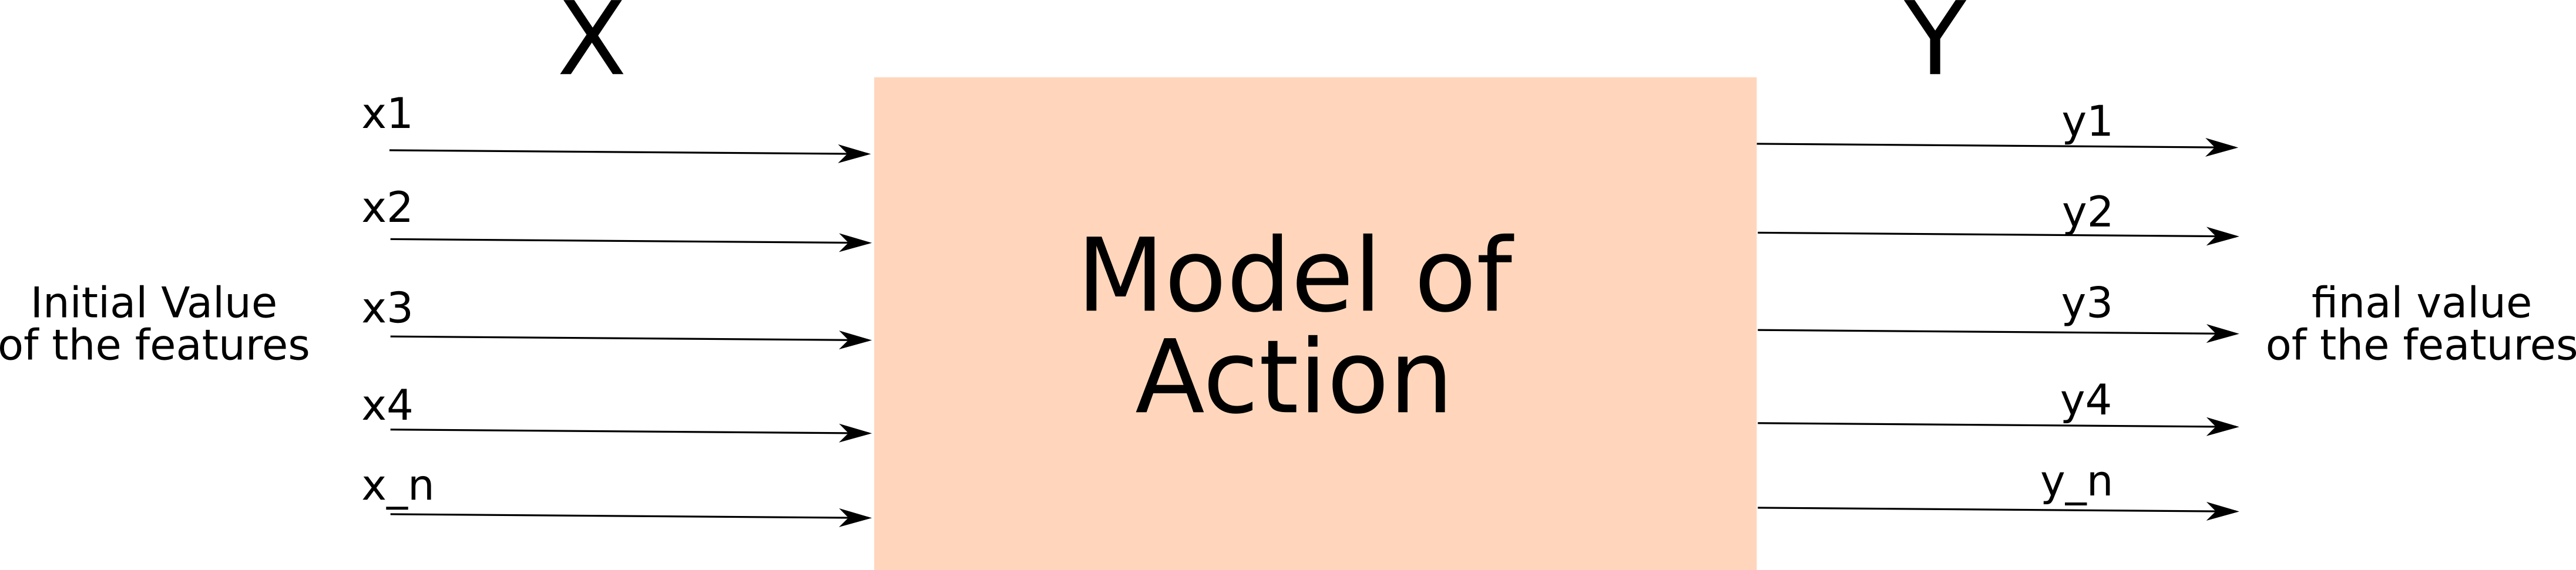
\includegraphics[scale=0.5]{/data/dataDeebul/rnd/RecommenderSystemInRobotics/art/modelAction.png}
\caption{Model Selection}
\label{Figure}
\end{figure}

The problem here can be taken as a supervised learning problem, where the model has to learn from the demonstrations and predict the output Y when the new input X is provided. The objective of the model is to Maximize the message conveyed to Y about X. 

\section{Entropy}

Consider a random variable X as a discrete random variable, modelled as 

\begin{equation}
    X = \{x_k | k = 0, \pm 1, ..., \pm K\}
\end{equation}

where the sample value $x_k$ is a discrete number and (2K + 1) is the total number of discrete levels.

Now let the event X = $x_k$ occur with probability
\begin{equation}
	p_k = P(X = x_k)
\end{equation}
with the requirement that 
\begin{equation}
	0 \leq p_k \leq 1 and \sum _{k = -K}^{K} = 1
\end{equation}

We define the amount of information gained after observing the event X = $x_k$ with probability $p_k$ as the logarithmic function 
\begin{equation}
	I(x_k) = \log(1 / p_k) = -\log(p_k)
\end{equation}
where the base of the logarithm is arbitrary. 

The amount of information $I(x_k)$ is a discrete random variable with probability $p_k$. The mean value of $I(x_k)$ over the complete range $2K +1$ discrete values is given by

\begin{align*}
	H(X) = \mathbb{E}[I(x_k)] \\
	     = \sum _{k = -K}^{K}p_k I(x_k)\\
	     = - \sum _{k = -K}^{K} p_k \log p_k
\end{align*}

The quantity $H(X)$ is called the entropy of a random variable $X$ permitted to take a finite set of discrete values.

The entropy $H(X)$ is a measure of the average amount of information conveyed per message. Note, however, that the $X$ in $H(X)$  is not an argument of a function, but rather a label for a random variable. Note also that in the equation we take 0 $\log$ 0 to be 0.

The entropy $H(X)$ is bounded as 
\begin{equation}
	0 \leq H(X) \leq \log(2K + 1)
\end{equation}
where  $2K + 1$ is the total number of discrete levels. Furthermore we can make 2 statements:

\begin{enumerate}
	\item $H(X) = 0$ if, and only if, the probability $p_k = 1$ for some k and the remaining probabilities in the set are all zero; this lower bound entropy corresponds to no uncertainty.
	\item $H(X) = \log(2K + 1)$, if, and only if, $p_k = 1 / (2K + 1)$ for all k ; this upper bound on entropy corresponds to maximum uncertainty.
	
\end{enumerate}


\end{document}